%  LaTeX support: latex@mdpi.com
%  In case you need support, please attach all files that are necessary for compiling as well as the log file, and specify the details of your LaTeX setup (which operating system and LaTeX version / tools you are using).

% You need to save the "mdpi.cls" and "mdpi.bst" files into the same folder as this template file.

%=================================================================
\documentclass[journal,article,submit,moreauthors,pdftex,10pt,a4paper]{mdpi} 

%--------------------
% Class Options:
%--------------------
% journal
%----------
% Choose between the following MDPI journals:
% actuators, admsci, aerospace, agriculture, agronomy, algorithms, animals, antibiotics, antibodies, antioxidants, applsci, arts, atmosphere, atoms, axioms, batteries, behavsci, beverages, bioengineering, biology, biomedicines, biomimetics, biomolecules, biosensors, brainsci, buildings, carbon, cancers, catalysts, cells, challenges, chemosensors, children, chromatography, climate, coatings, computation, computers, condensedmatter, cosmetics, cryptography, crystals, data, dentistry, designs, diagnostics, diseases, diversity, econometrics, economies, education, electronics, energies, entropy, environments, epigenomes, fermentation, fibers, fishes, fluids, foods, forests, futureinternet, galaxies, games, gels, genealogy, genes, geosciences, geriatrics, healthcare, horticulturae, humanities, hydrology, informatics, information, infrastructures, inorganics, insects, instruments, ijerph, ijfs, ijms, ijgi, inventions, jcdd, jcm, jdb, jfb, jfmk, jimaging, jof, jintelligence, jlpea, jmse, jpm, jrfm, jsan, land, languages, laws, life, literature, lubricants, machines, magnetochemistry, marinedrugs, materials, mathematics, mca, mti, medsci, medicines, membranes, metabolites, metals, microarrays, micromachines, microorganisms, minerals, molbank, molecules, mps, nanomaterials, ncrna, neonatalscreening, nutrients, particles, pathogens, pharmaceuticals, pharmaceutics, pharmacy, philosophies, photonics, plants, polymers, processes, proteomes, publications, recycling, religions, remotesensing, resources, risks, robotics, safety, sensors, separations, sexes, sinusitis, socsci, societies, soils, sports, standards, sustainability, symmetry, systems, technologies, toxics, toxins, universe, urbansci, vaccines, vetsci, viruses, water
%---------
% article
%---------
% The default type of manuscript is article, but can be replaced by: 
% addendum, article, book, bookreview, briefreport, casereport, changes, comment, commentary, communication, conceptpaper, correction, conferencereport, expressionofconcern, meetingreport, creative, datadescriptor, discussion, editorial, essay, erratum, hypothesis, interestingimage, letter, newbookreceived, opinion, obituary, projectreport, reply, retraction, review, sciprints, shortnote, supfile, technicalnote
% supfile = supplementary materials
%----------
% submit
%----------
% The class option "submit" will be changed to "accept" by the Editorial Office when the paper is accepted. This will only make changes to the frontpage (e.g. the logo of the journal will get visible), the headings, and the copyright information. Also, line numbering will be removed. Journal info and pagination for accepted papers will also be assigned by the Editorial Office.
%------------------
% moreauthors
%------------------
% If there is only one author the class option oneauthor should be used. Otherwise use the class option moreauthors.
%---------
% pdftex
%---------
% The option pdftex is for use with pdfLaTeX. If eps figure are used, remove the option pdftex and use LaTeX and dvi2pdf.

%=================================================================
\firstpage{1} 
\makeatletter 
\setcounter{page}{\@firstpage} 
\makeatother 
\articlenumber{x}
\doinum{10.3390/------}
\pubvolume{xx}
\pubyear{2016}
\copyrightyear{2016}
\externaleditor{Academic Editor: name}
\history{Received: date; Accepted: date; Published: date}
%------------------------------------------------------------------
\usepackage{caption} 
\usepackage{hhline} % para usar linha dupla na tabela
\usepackage{tabularx} % para igualar colunas
\usepackage{dcolumn} % para efetuar alinhamento
\usepackage{amsmath}
\usepackage[table,xcdraw]{xcolor}
\usepackage{graphicx}      % include this line if your document contains figures
\usepackage{indentfirst}
\usepackage{subfigure}
% The following line should be uncommented if the LaTeX file is uploaded to arXiv.org
%\pdfoutput=1

%=================================================================
% Add packages and commands here. The following packages are loaded in our class file: fontenc, calc, indentfirst, fancyhdr, graphicx, lastpage, ifthen, lineno, float, amsmath, setspace, enumitem, mathpazo, booktabs, titlesec, etoolbox, amsthm, hyphenat, natbib, hyperref, footmisc, geometry, caption, url, mdframed

%=================================================================
%% Please use the following mathematics environments:
 \theoremstyle{mdpi}
 \newcounter{thm}
 \setcounter{thm}{0}
 \newcounter{ex}
 \setcounter{ex}{0}
 \newcounter{re}
 \setcounter{re}{0}

 \newtheorem{Theorem}[thm]{Theorem}
 \newtheorem{Lemma}[thm]{Lemma}
 \newtheorem{Corollary}[thm]{Corollary}
 \newtheorem{Proposition}[thm]{Proposition}

 \theoremstyle{mdpidefinition}
 \newtheorem{Characterization}[thm]{Characterization}
 \newtheorem{Property}[thm]{Property}
 \newtheorem{Problem}[thm]{Problem}
 \newtheorem{Example}[ex]{Example}
 \newtheorem{ExamplesandDefinitions}[ex]{Examples and Definitions}
 \newtheorem{Remark}[re]{Remark}
 \newtheorem{Definition}[thm]{Definition}
%% For proofs, please use the proof environment (the amsthm package is loaded by the MDPI class).

%=================================================================
% Full title of the paper (Capitalized)
\Title{Classificação dos níveis de maturação do tomate Caline IPA-06 através do processamento de imagens}

% Authors, for the paper (add full first names)
\Author{Luiz Diego Vidal $^{1,\dagger,\ddagger}$,Adilson Enes$^{2,\ddagger}$,Silvestre Rodrigues$^{3,\ddagger}$,Luiz Fernando Ganassali $^{4,\ddagger}$, Airton Marques $^{5,\ddagger}$ and Igor Sabino $^{6,\ddagger}$}
% Authors, for metadata in PDF
\AuthorNames{Luiz Diego Vidal, Adilson Machado Enes, Luiz Fernando Ganassali de Oliveira Junior, Airton Marques and Igor Sabino}

% Affiliations / Addresses (Add [1] after \address if there is only one affiliation.)
\address{%
$^{1}$ \quad Universidade Federal de Sergipe, SE 49100-000 BR; vidal.center@academico.ufs.br\\
$^{2}$ \quad Universidade Federal de Sergipe, SE 49100-000 BR; adilsonenes@gmail.com\\
$^{3}$ \quad Universidade Federal de Sergipe, SE 49100-000 BR; silvestrerod@yahoo.com.br\\
$^{4}$ \quad Universidade Federal de Sergipe, SE 49100-000 BR; lfg.ufs@gmail.com\\
$^{5}$ \quad Universidade Federal de Sergipe, SE 49100-000 BR; airtonsocial@hotmail.com\\
$^{6}$ \quad Universidade Federal de Sergipe, SE 49100-000 BR; igorsabrabe@gmail.com}

% Contact information of the corresponding author
\corres{Correspondence: vidal.center@academico.ufs.br; Tel.: +55(079) 996467276}

% Current address and/or shared authorship
%\firstnote{Current address: Affiliation 3} 
%\secondnote{These authors contributed equally to this work.}
% Simple summary
%\simplesumm{}

% Abstract (Do not use inserted blank lines, i.e. \\) 
\abstract{Parâmetros fisiológicos como acidez, massa, e cor destacam-se como indicadores de maturação em tomates, porém exigem tempo e trabalho para medições.A possibilidade de usar a Processamento de imagens (PDI) associados aos sistemas de previsão desses
variáveis fisiológicas podem auxiliar na predição e manutenção da qualidade dos tomates após a colheita de forma mais rápida e não invasiva. Com este objetivo, foi realizado um experimento com tomates Caline IPA-06, delineados experimentalmente ao acaso utilizando cinco repetições durante cinco períodos de maturação (0, 3, 6, 9 e 12 dias). Foram avaliadas as variáveis: Acidez titulável, PH, Sólidos solúveis, Massa fresca e Cor. Para analise da atividade biológica através do PDI foi utilizado o método biospeckle laser através das técnicas de Momento de Inercia (MI) e Diferença Generalizada (DG), todas sobre filtragem com aberturas de janelas através do filtro Wavelet. 
Nos resultados obtidos através deste modelo de simulação em PDI, quando comparado com demais evidenciaram existir correlação com a diminuição na taxa da atividade biológica e a perda de massa fresca. As amostras apresentaram mudanças significativas, para sólidos solúveis, cor  e PH mas estas não demostraram correlação com o comportamento do biospeckle.}

% Keywords
\keyword{\textit{Lycopersicon esculentum}, Pós-colheita, Biospeckle Laser.}

% The fields PACS, MSC, and JEL may be left empty or commented out if not applicable
%\PACS{J0101}
%\MSC{}
%\JEL{}

% If this is an expanded version of a conference paper, please cite it here: enter the full citation of your conference paper, and add $^\S$ in the end of the title of this article.
%\conference{}

%%%%%%%%%%%%%%%%%%%%%%%%%%%%%%%%%%%%%%%%%%
% Only for the journal Data:

%\dataset{DOI number or link to the deposited data set in cases where the data set is published or set to be published separately. If the data set is submitted and will be published as a supplement to this paper in the journal Data, this field will be filled by the editors of the journal. In this case, please make sure to submit the data set as a supplement when entering your manuscript into our manuscript editorial system.}

%\datasetlicense{license under which the data set is made available (CC0, CC-BY, CC-BY-SA, CC-BY-NC, etc.)}

%%%%%%%%%%%%%%%%%%%%%%%%%%%%%%%%%%%%%%%%%%
\begin{document}

%%%%%%%%%%%%%%%%%%%%%%%%%%%%%%%%%%%%%%%%%%
%% Sections that are not mandatory are listed as such. The section titles given are for Articles. Review papers and other article types have a more flexible structure. 

%% Only for the journal Gels: Please place the Experimental Section after the Conclusions

%%%%%%%%%%%%%%%%%%%%%%%%%%%%%%%%%%%%%%%%%%

\section{Introduction}
Este trabalho baseia-se na ocorrência de um fenômeno óptico conhecido na física como speckle dinâmico, tendo sua nomenclatura, sofrido alterações à medida que se descobriu novas aplicações para o mesmo, atualmente é conhecido como biospeckle dinâmico. \citep{Rodrigues2007} entre outros autores, descreve o fenômeno da seguinte forma:
“O biospeckle ou speckle dinâmico é um fenômeno óptico de interferência que ocorre quando há incidência de luz coerente em materiais, cujas superfícies sejam opticamente rugosas e que possuem algum tipo de atividade."

O embasamento teórico e experimental aponta no sentido de que é possível identificar à frequência em que biospeckle sofre interferência da variação do comportamento do fruto em relação a mudanças durante a maturação \cite{Zdunek2014}. Em materiais biológicos, os níveis de atividades estão diretamente relacionados com a viabilidade celular, troca de gases, respiração, atividade microbiana e atividade de água (aw). 
 Por esta razão, o fenômeno tem sido estudado como uma potencial ferramenta na análise de qualidade e viabilidade de diversos materiais biológicos, como a viabilidade de sêmen bovino \cite{Henrique2007a}, viabilidade de sementes arbóreas \citep{Aparecida2011} e qualidade de frutos \citep{Cotching2018}.

% aqui inicia a parte de tomates
O tomateiro é uma planta de ciclo curto, do tipo climatérico e sofre com diversas alterações em sua característica em relação a cor \citep{santana2017infodengue}, firmeza, aroma, e sabor \citep{CarmeloLuisGustavoPaulino;FerreiraMarcosDavid;GimenezCalbo2015} ao logo de sua vida útil 
A tomaticultura apresenta altas perdas da qualidade, as quais ocorrem do plantio até o consumo final. Com relação a estas perdas, diversos métodos de análise foram elaborados buscando um melhor controle da qualidade ideal. 

% aqui inicia a parte da eng. agrí
Sabe-se que os avanços mais notáveis no campo de máquinas agrícolas dos últimos tempos têm se dado no campo da agricultura de precisão, que busca ser feita de forma precisa nos parâmetros e variáveis responsáveis por influenciar toda cadeia produtiva, como por exemplo, o tempo de prateleira dos frutos. Para atingir este propósito, sensores são instalados em máquinas, permitindo que os dados referentes à qualidade sejam comparados com outros fatores, o que possibilita um controle mais efetivo, preciso e econômico.
Diante dos fatos apresentados, este artigo visou propor o estudo e modelamento da atividade de maturação do tomate IPA6 corroborando com métodos utilizados atualmente. Este conhecimento será importante, pois no futuro, poderá ser usado para o desenvolvimento de sensores que permitirão indicar de forma indireta, a qualidade do fruto, bem como seu tempo de prateleira, contribuindo para a agregação de valor no mercado comercial de hortaliças. 

%%%%%%%%%%%%%%%%%%%%%%%%%%%%%%%%%%%%%%%%%%
\section{Results}

Os valores de Momento de Inercia capturados pelo método de biospeckle dinâmico apresentaram diferença significativa, valores constantes na Tabela 2. Com relação ao comportamento da regressão, os primeiros níveis demonstraram um comportamento linear.

%tabela para massa
\begin{table}[ht]\footnotesize
\centering
\caption{Análise de Variância com significância a 5\% para perda de Massa Fresca}
\label{anova_massa}
\begin{tabular}{|c|l|l|l|l|l|l|}
\hline
Fonte de variação & SQ       & gl & MQ         & F           & valor P                         \\ \hline
Entre grupos      & 317,5684 & 4  & 79,3921   & 0,556925424 & {\color[HTML]{FD6864} 0,69641138}\\ \hline
Dentro de grupos  & 2851,0855 & 20 & 142,554275 &             &                            \\ \hline
\end{tabular}
\end{table}

% tabela para MI
\begin{table}[ht]\footnotesize
\centering
\caption{Análise de Variância com significância a 5\% para Momento de Inércia}
\label{anova_mi}
\begin{tabular}{|c|l|l|l|l|l|l|}
\hline
Fonte de variação & SQ       & gl & MQ         & F           & valor P                            \\ \hline
Entre grupos& 245,81444 & 4  & 61,453610  & 3,127652197 & {\color[HTML]{FD6864} 0,0376379}\\ \hline
Dentro de grupos  & 392,96959 & 20 & 19,64847951
 &             &                            \\ \hline
\end{tabular}
\end{table}

%regressões
\begin{figure}[!htb]  
\centering
\subfigure[ref1][Regressão para perda de massa fresca]{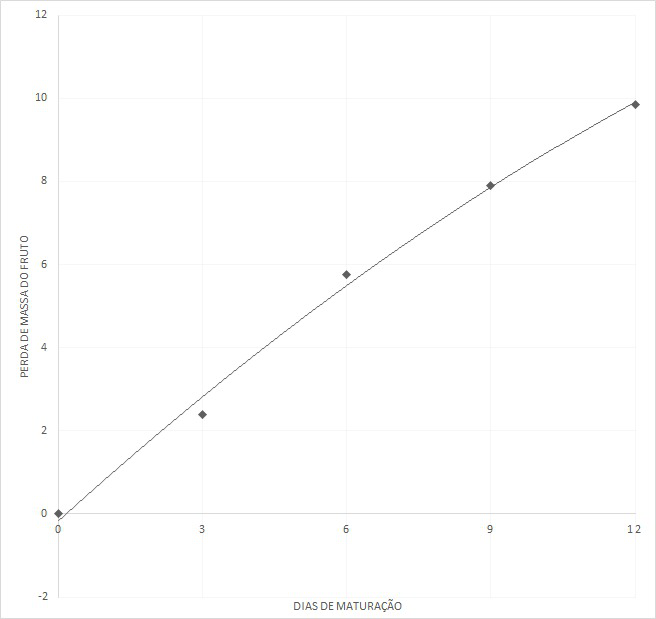
\includegraphics[width=4cm]{figure/estatistica/regressao_massa.png}}
\qquad
\subfigure[ref2][Regressão de atividades do Momento de Inercia]{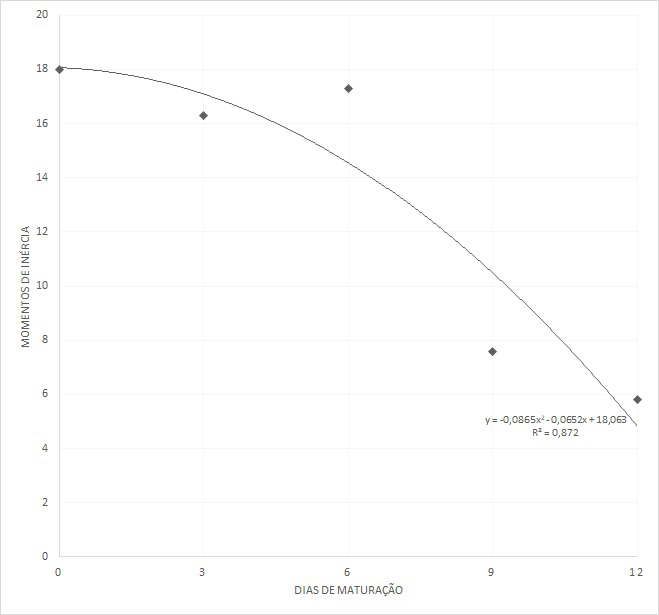
\includegraphics[width=4cm]{figure/estatistica/regressao_inercia.png}}
\caption{(a) Regressão perda de massa fresca e (b) Regressão MI.}
\label{regressao_MI_massa}
\end{figure}

\begin{figure}[!htb]  
\centering
\subfigure[ref1][Regressão para sólidos solúveis]{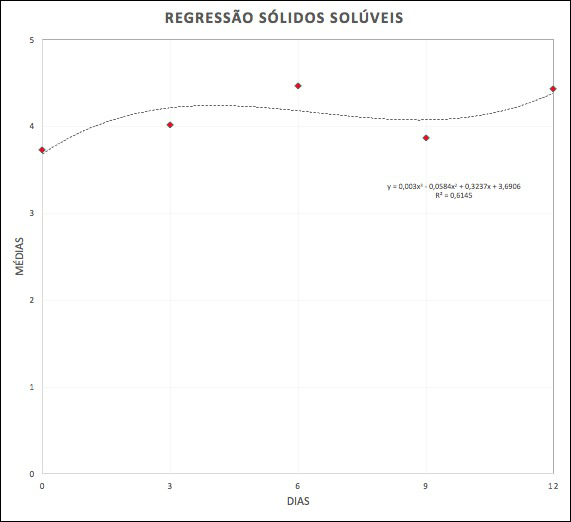
\includegraphics[width=4cm]{figure/estatistica/regressao_soluveis.png}}
\qquad
\subfigure[ref2][Regressão de atividades do Momento de Inercia]{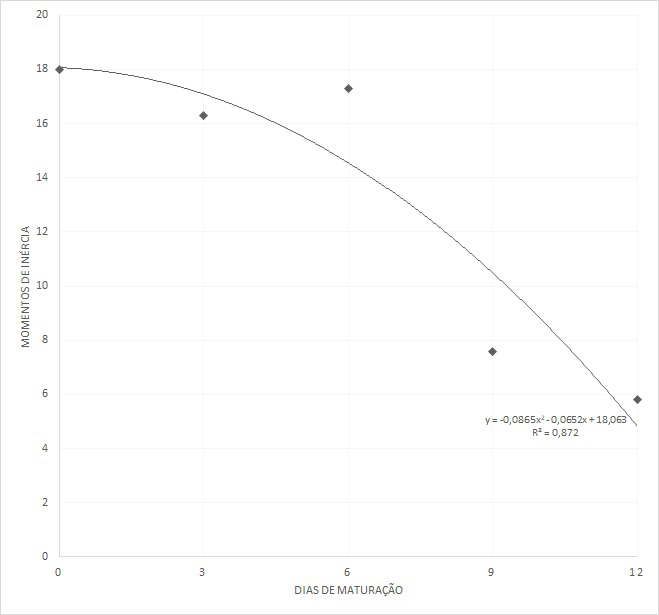
\includegraphics[width=4cm]{figure/estatistica/regressao_inercia.png}}
\caption{(a) Regressão sólidos solúveis (b) Regressão MI.}
\label{regressao_solido}
\end{figure}

\begin{figure}[!htb]  
\centering
\subfigure[ref1][Regressão para firmeza dos frutos]{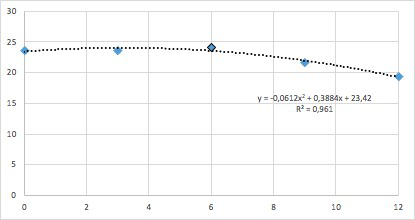
\includegraphics[width=4cm]{figure/estatistica/regressao_firmeza.png}}
\qquad
\subfigure[ref2][Regressão de atividades do Momento de Inercia]{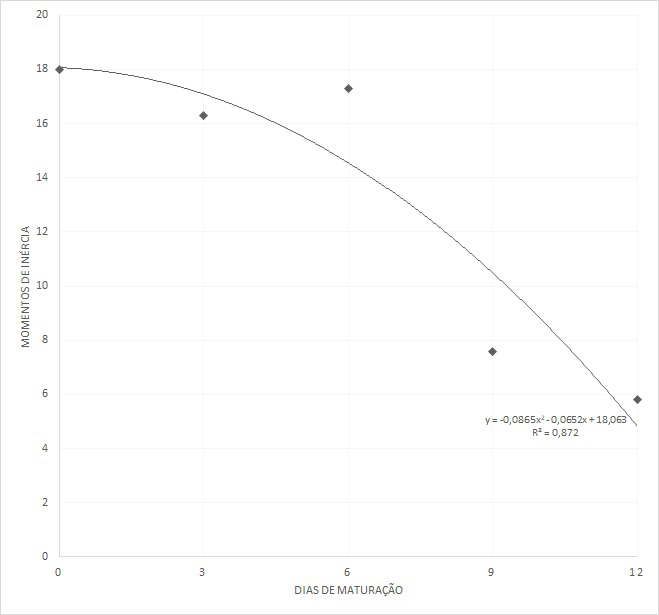
\includegraphics[width=4cm]{figure/estatistica/regressao_inercia.png}}
\caption{(a) Regressão Firmeza dos frutos (b) Regressão MI.}
\label{regressao_firmeza}
\end{figure}

\newpage
\subsection{Mapeamento de frequências por testes preliminares de Fourier e Wavelets}

Os dados mostram haver correlação entre a perda de massa fresca das amostas e os níveis de atividade monitorados pelo biospeckle laser, conforme pode ser observados nos diferentes níveis. Partido da Figura \ref{atividades1}a à Figura  \ref{atividades5}a, resultantes do processamento com o  método DG  e reconstrução de uma única banda de frequência. Onde nos valores mais altos representados didaticamente na \ref{atividades1}a apresentam altas atividades, representados pelas cores amarelo e verde, tons mais quentes, já a Figura \ref{atividades5}a os tons se apresentam mais baixos, mais próximos dos azul e cinza, cores mais frias, demonstrando que o nível de atividade teve uma ligeira queda. Para os dados referentes ao MI, utilizamos o modelo virtual de Momento de Ocorrência Modificada para demonstrar a amplitude das atividades, neste modelo o fache de pixels brancos que desenha uma linha inclinada ao quadro demostra que quanto mais dispersos os pontos, maior a atividade registrada Figura \ref{atividades1}b, e o contrário (mais organizados e próximos a linha inclinada) menor é o registro de atividade, Figura \ref{atividades5}b. O uso de apenas uma banda para o processamento com o DG demonstrou seletividade em diferentes níveis de massa. \citep{Zdunek2014} demostrou haver influência dos diferentes níveis de água em grãos de milho influenciam as taxas de atividades registradas pelo biospeckle onde, o grão com presenças de rachaduras e conseguinte maior evaporação da água apresentou níveis maiores de atividade que os grão que não apresentaram rachaduras, corroborando com este experimento, haja vista que, quanto maior a presença da água no material biológico,  maior os níveis de biospeckle. Utilizando a Analise de Variância (ANOVA) com o teste de Tukey com o nível de significância a 5\%, não ouve diferença significativa  entre os diferentes níveis de massa durante os períodos de maturação, como pode ser observado na figura \ref{regressao_MI_massa} porém, observando o comportamento dos gráficos de dispersão para perda de massa e momento de inércia, podemos verificar uma tendencia.


\begin{figure}[!htb]  
\centering
\subfigure[ref1][Diferença Generalizada ]{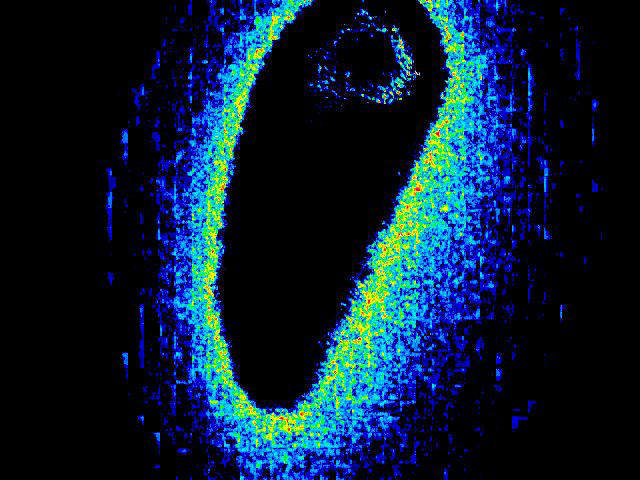
\includegraphics[width=4cm]{figure/dgs/dia_1.png}}
\qquad
\subfigure[ref2][Momento de Ocorrência Modificada]{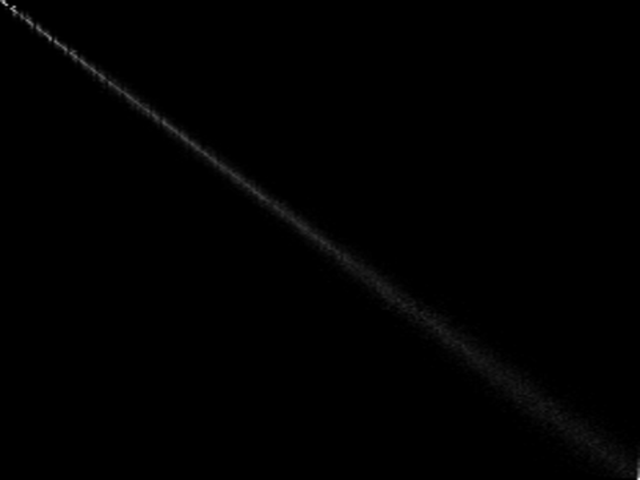
\includegraphics[width=4cm]{figure/moc/dia_1.png}}
\caption{(a) Diferença Generalizada tratamento (0 dia) e Momento de Ocorrência Modificada (0 dias).}
\label{atividades1}
\end{figure}

\begin{figure}[!htb]
\centering
\subfigure[ref3][Diferença Generalizada 3 Dia]{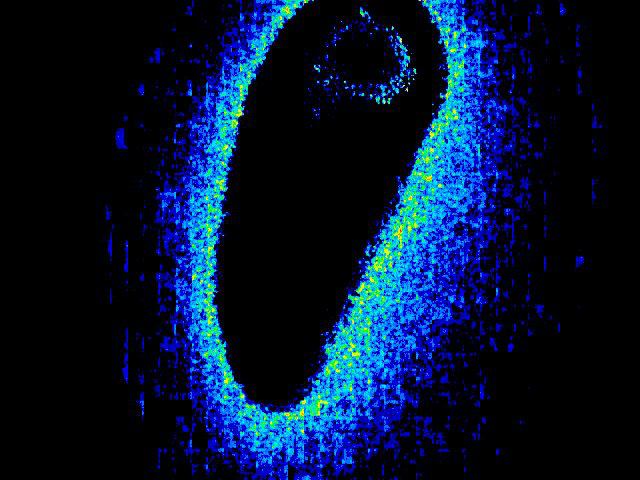
\includegraphics[width=4cm]{figure/dgs/dia_2.png}}
\qquad
\subfigure[ref4][Momento de Ocorrência Modificada]{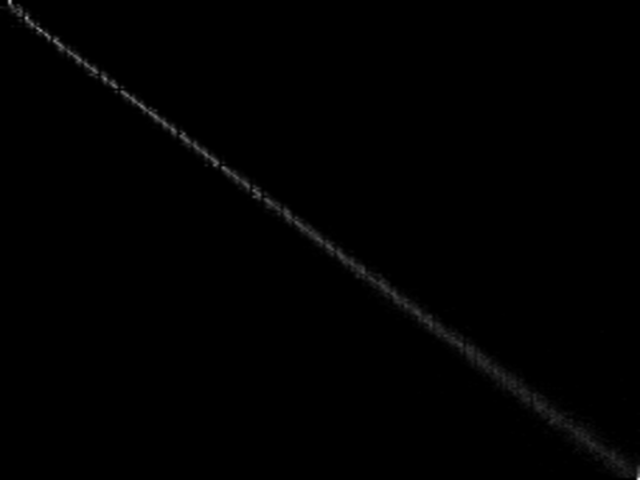
\includegraphics[width=4cm]{figure/moc/dia_4.png}}
\caption{(a) Diferença Generalizada tratamento (3 dia) e Momento de Ocorrência Modificada (3 dias) .}
\label{atividades2}
\end{figure}

\begin{figure}[!htb]
\centering
\subfigure[ref3][Diferença Generalizada ]{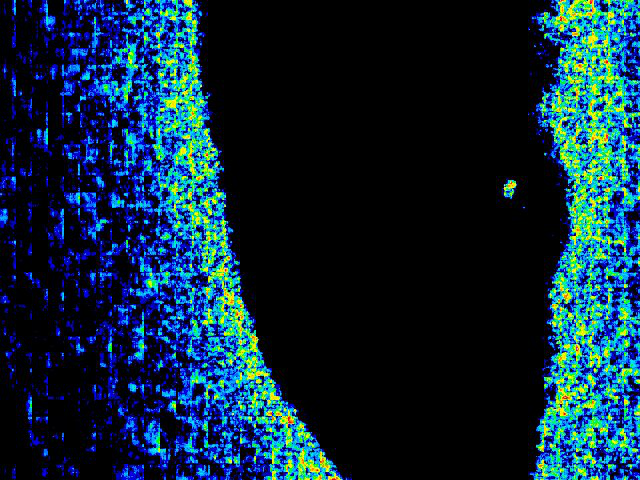
\includegraphics[width=4cm]{figure/dgs/dia_3.png}}
\qquad
\subfigure[ref4][Momento de Ocorrência Modificada Dia 0]{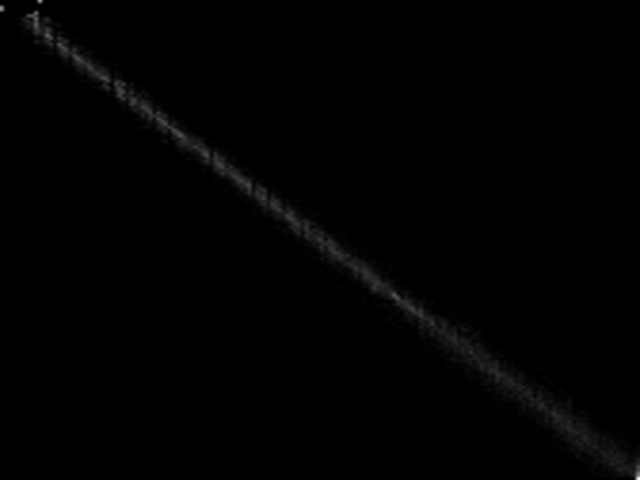
\includegraphics[width=4cm]{figure/moc/dia_3.png}}
\caption{(a) Diferença Generalizada tratamento (6 dia) e Momento de Ocorrência Modificada (6 dias) .}
\label{atividades3}
\end{figure}


\begin{figure}[!htb]
\centering
\subfigure[ref3][Diferença Generalizada ]{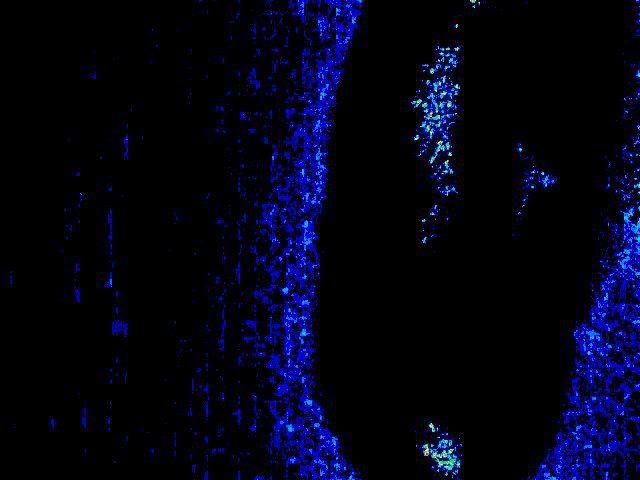
\includegraphics[width=4cm]{figure/dgs/dia_4.png}}
\qquad
\subfigure[ref4][Momento de Ocorrência Modificada]{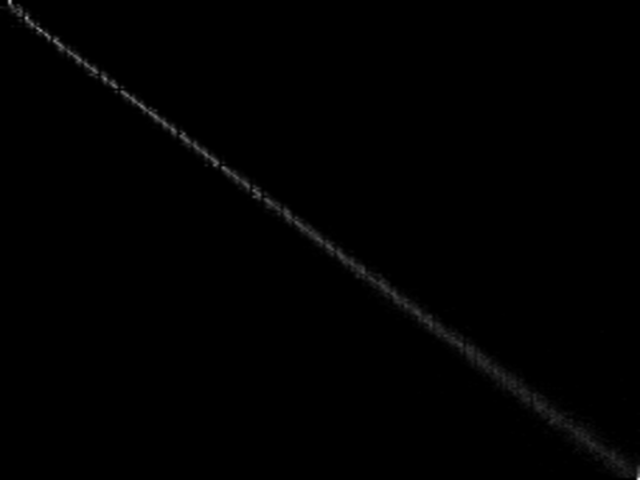
\includegraphics[width=4cm]{figure/moc/dia_4.png}}
\caption{(a) Diferença Generalizada tratamento (9 dias) e Momento de Ocorrência Modificada (9 dias) .}
\label{atividades4}
\end{figure}

\begin{figure}[!htb]
\centering
\subfigure[ref3][Diferença Generalizada ]{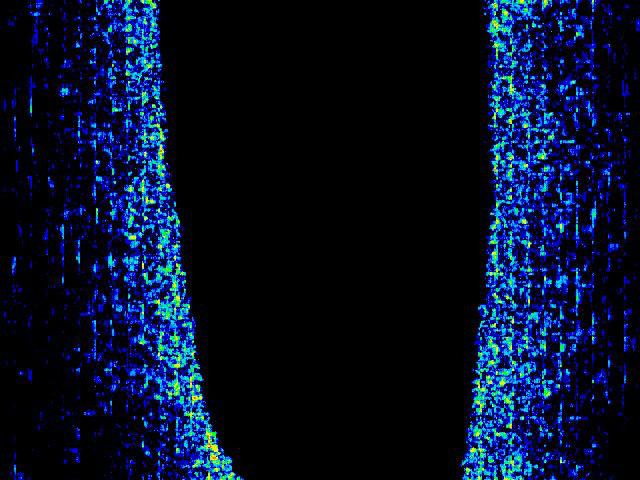
\includegraphics[width=4cm]{figure/dgs/dia_5.png}}
\qquad
\subfigure[ref4][Momento de Ocorrência Modificada]{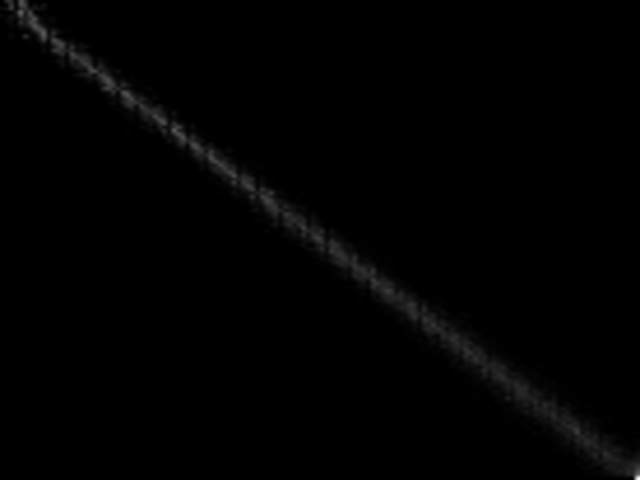
\includegraphics[width=4cm]{figure/moc/dia_5.png}}
\caption{(a) Diferença Generalizada tratamento (12 dias) e Momento de Ocorrência Modificada (12 dias) .}
\label{atividades5}
\end{figure}

\newpage

\section{Discussion}

This section may be divided by subheadings. Authors should discuss the results and how they can be interpreted in perspective of previous studies and of the working hypotheses. The findings and their implications should be discussed in the broadest context possible. Future research directions may also be highlighted.

%%%%%%%%%%%%%%%%%%%%%%%%%%%%%%%%%%%%%%%%%%
\section{materials and methods}
\subsection{Análises físico-químicas} 

Para  determinação da acidez total titulável e sólidos solúveis totais foram utilizadas as metodologias descritas por \citep{Graca2015}. Quanto a Firmeza e cor das amostras foram utilizados métodos descritos por \citep{Horwitz}, levando em consideração que para firmeza foi utilizada a ponteira de prova com 8mm de diamentro e para coloração o sistema L*a*b*.

%\newpage


\subsection{Delineamento Experimental}
O delineamento experimental foi interamente casualizado contando com cinco tratamentos (0, 3, 6, 9 e 12 dias) e cinco repetições. As amostras foram selecionadas conforme a cor de maturação (verde). 
\subsubsection{Methodology for image capture}
Com o Lazer HeNe 632nm incidindo nas amostras de solo \ref{fig:laser}, foram coletadas imagens através de método direto que consistia dos vídeos  direto da câmera através de um cabo AVI e uma conectado em uma placa de vídeo assim, a aquisição dos frames através da quebra do vídeo já roda diretamente no software principal da pesquisa com um intervalo de 0.15 segundos para as aquisições que equivale o tempo de aquisição da câmera para cada frame, evitando assim a interpolação de imagens, a perda de arquivos e principalmente a interferência durante a coleta das imagens.

%setup da captura das imagens biospeckle
\begin{figure}[htb]
\centering
\subfigure[ref5][Análise biospeckle Laser]{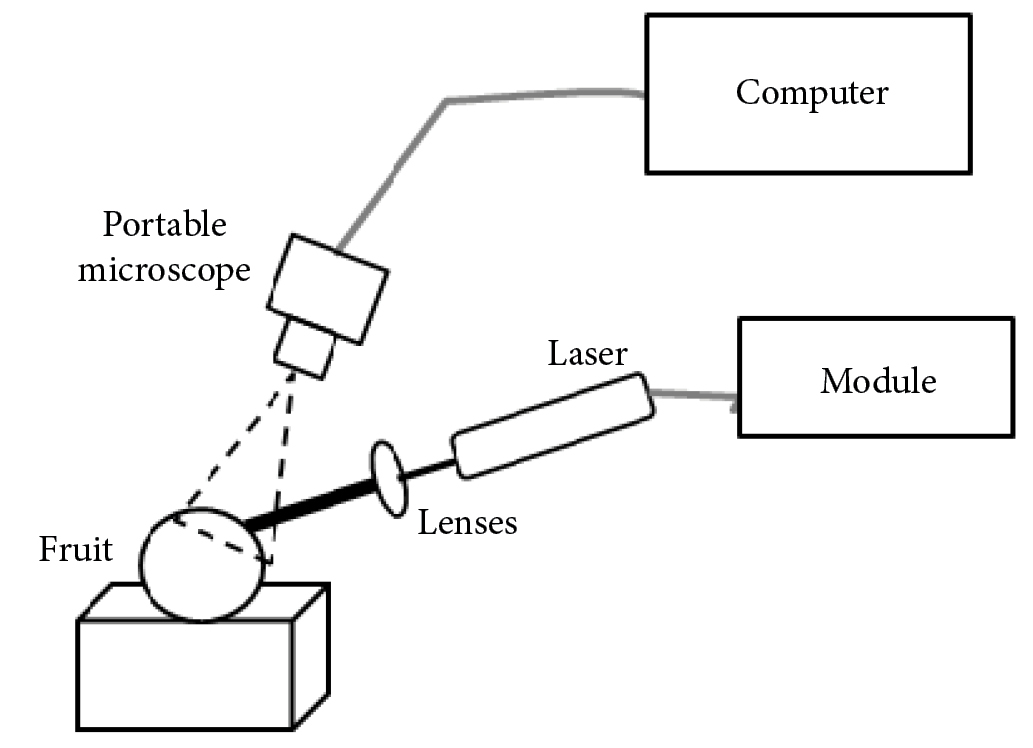
\includegraphics[width=4cm]{figure/materiais/setup.png}}
\caption{Setup para aquisição de imagens.}
\label{fig:laser}
\end{figure}


\subsection{Analise estatística}

Para a avaliação da normalidade dos dados foi utilizado o teste de Normalidade Shapiro Wilk (SK) os dados que seguiram a normalidade foi utilizado método de analise de variância de um fator (ANOVA) e o teste de Tukey para comparações multiplas, para os que não seguiram a normalidade foi utilizado Teste de Kruskal-Wallis. As médias, a partir dos dados obtidos , foram submetidas regressão buscando analisar o comportamento sob a perspectiva de progressão do tempo de maturação, foi testado os modelos lineares e polinomial, considerando o melhor ajuste com R2 ≥ 80\%.


%%%%%%%%%%%%%%%%%%%%%%%%%%%%%%%%%%%%%%%%%%
\section{Conclusions}

Este trabalho apresentou resultados favoráveis ao avaliar não-destrutivamente os níveis de maturação do tomate Caline IPA-06 através do uso de processamento de imagens baseado no biospeckle dinâmico associando-as a métodos rotineiros e numéricos. Tanto para amostragem espectral tendo como base o DG ou amostragem numérica baseado no MI. Descobrimos que o momento de inércia em segunda ordem (MI) é sensível a mudança nos níveis de massa fresca, conforme se perde a quantidade de massa do fruto se reduziu a ocorrência do fenômeno.
%\supplementary{The following are available online at www.mdpi.com/link, Figure S1: title, Table S1: title, Video S1: title.}
%%%%%%%%%%%%%%%%%%%%%%%%%%%%%%%%%%%%%%%%%%
\acknowledgments{All sources of funding of the study should be disclosed. Please clearly indicate grants that you have received in support of your research work. Clearly state if you received funds for covering the costs to publish in open access.}

%%%%%%%%%%%%%%%%%%%%%%%%%%%%%%%%%%%%%%%%%%
\authorcontributions{For research articles with several authors, a short paragraph specifying their individual contributions must be provided. The following statements should be used ``X.X. and Y.Y. conceived and designed the experiments; X.X. performed the experiments; X.X. and Y.Y. analyzed the data; W.W. contributed reagents/materials/analysis tools; Y.Y. wrote the paper.'' Authorship must be limited to those who have contributed substantially to the work reported.}

%%%%%%%%%%%%%%%%%%%%%%%%%%%%%%%%%%%%%%%%%%
\conflictofinterests{Declare conflicts of interest or state ``The authors declare no conflict of interest.'' Authors must identify and declare any personal circumstances or interest that may be perceived as inappropriately influencing the representation or interpretation of reported research results. Any role of the funding sponsors in the design of the study; in the collection, analyses or interpretation of data; in the writing of the manuscript, or in the decision to publish the results must be declared in this section. If there is no role, please state ``The founding sponsors had no role in the design of the study; in the collection, analyses, or interpretation of data; in the writing of the manuscript, and in the decision to publish the results''.} 

%%%%%%%%%%%%%%%%%%%%%%%%%%%%%%%%%%%%%%%%%%
%% optional
\abbreviations{The following abbreviations are used in this manuscript:\\

\noindent MDPI: Multidisciplinary Digital Publishing Institute\\
DOAJ: Directory of open access journals\\
TLA: Three letter acronym\\
LD: linear dichroism}

%%%%%%%%%%%%%%%%%%%%%%%%%%%%%%%%%%%%%%%%%%
%% optional
\appendix
\section{}
The appendix is an optional section that can contain details and data supplemental to the main text. For example, explanations of experimental details that would disrupt the flow of the main text, but nonetheless remain crucial to understanding and reproducing the research shown; figures of replicates for experiments of which representative data is shown in the main text can be added here if brief, or as Supplementary data. Mathemtaical proofs of results not central to the paper can be added as an appendix.

\section{}
All appendix sections must be cited in the main text. In the appendixes, Figures, Tables, etc. should be labeled starting with `A', e.g., Figure A1, Figure A2, etc. 

%%%%%%%%%%%%%%%%%%%%%%%%%%%%%%%%%%%%%%%%%%
\bibliographystyle{mdpi}
\bibliography{mendeley}
%=====================================
% References, variant A: internal bibliography
%=====================================

%%%%%%%%%%%%%%%%%%%%%%%%%%%%%%%%%%%%%%%%%%
\end{document}

